\documentclass{ximera}

\usepackage{float}

\newcommand{\R}{\mathbb R}

\newcommand{\href}[2]{#2\footnote{\url{#1}}}
\newcommand{\verticalvector}[1]{\begin{bmatrix}#1\end{bmatrix}}
\newcommand{\gt}{>}

\pgfplotsset{compat=1.8}
\graphicspath{
{./}
{introduction/}
{unit1/}
{unit1/theGeometryOfLinearEquations/}
{unit1/EliminationwithMatrices/}
{unit1/MultiplicationandInverseMatrices/}
}


\title{Factorization into A = LU}

\begin{document}
\begin{abstract}
  Unit 1 MIT OCW Linear Algebra: Factorization into A = LU
\end{abstract}
\maketitle

The MIT OCW Video Lecture can be found
here:\video{https://www.youtube.com/watch?v=5hO3MrzPa0A}\\

This session explains inverses, transposes and permutation matrices. We also learn how elimination leads to a useful factorization A = LU and how hard a computer will work to invert a very large matrix.

\begin{figure}[H]
\begin{image}
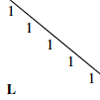
\includegraphics{1_4.jpg}
\end{image}
\end{figure}

One goal of today?s lecture is to understand Gaussian elimination in terms of matrices; to find a matrix $L$ such that $A = LU$. We start with some useful facts about matrix multiplication.

\section*{Inverse of a product}

The inverse of a matrix product $AB$ is $B_{?1} A_{?1}$.

\section*{Transpose of a product}

We obtain the transpose of a matrix by exchanging its rows and columns. In other words, 
the entry in row i column j of $A$ is the entry in row j column i of $A^T$.

The transpose of a matrix product $AB$ is $B^TA^T$. For any invertible matrix A, 
the inverse of $A^T$ is $(A^{-1})^T$

$A = LU$

We?ve seen how to use elimination to convert a suitable matrix $A$ into an upper 
triangular matrix $U$. This leads to the factorization $A = LU$, which is very helpful
in understanding the matrix $A$.

Recall that (when there are no row exchanges) we can describe the elimi�nation of the entries of matrix $A$ in terms of multiplication by a succession of elimination matrices $E_{ij}$, so that 
$A \rightarrow E21A  \rightarrow E_{31}E_{21}A  \rightarrow \cdots \rightarrow U$. In the two by two case this looks like:


\begin {table}[ht]
\centering
\begin {tabular} {c c c c}
$E_{21}$&$A$& &$U$\\
$\begin{bmatrix}  \phantom{-}1&0\\-4&1\end{bmatrix}$&$\begin{bmatrix} 2&1\\8&7\end{bmatrix}$&=&
$\begin{bmatrix} 2&1\\0&3\end{bmatrix}$
\end {tabular}
\end {table}

We can convert this to a factorization $A = LU$ by "canceling" the matrix $E_{21}$;
multiply by its inverse to get $E_{21}^{-1}E_{21}A = E_{21}^{-1}U$.

\begin {table}[ht]
\centering
\begin {tabular} {c c c c}
$A$& &$L$&$U$\\
$\begin{bmatrix} 2&1\\8&7\end{bmatrix}$&=&$\begin{bmatrix} 1&0\\4&1\end{bmatrix}$&
$\begin{bmatrix} 2&1\\0&3\end{bmatrix}$
\end {tabular}
\end {table}

The matrix $U$ is upper triangular with pivots on the diagonal. The matrix $L$ is lower 
triangular and has ones on the diagonal. Sometimes we will also want to factor out a 
diagonal matrix whose entries are the pivots:

\begin {table}[ht]
\centering
\begin {tabular} {c c c c c}
$A$& &$L$&$D$&$U^{'}$ \\
$\begin{bmatrix}  2&1\\8&7\end{bmatrix}$&=&$\begin{bmatrix} 1&0\\4&1\end{bmatrix}$&
$\begin{bmatrix} 2&0\\0&3\end{bmatrix}$&
$\begin{bmatrix} 1&\frac{1}{2}\\0&1\end{bmatrix}$
\end {tabular}
\end {table}

In the three dimensional case, if $E_{32}E_{31}E_{21}A = U$ then 
$A = E_{21}^{-1}E_{31}^{-1}E_{32}^{-1}U = LU$.

For example, suppose $E_{31}$ is the identity matrix and $E_{32}$ and $E_{21}$ are as
shown below:

\begin {table}[ht]
\centering
\begin {tabular} {c c c c}
$E_{32}$&$E_{21}$&$ $&$E$ \\
$\begin{bmatrix}  1&\phantom{-}0&0\\0&\phantom{-}1&0\\0&-5&1\end{bmatrix}$&
$\begin{bmatrix} \phantom{-}1&0&0\\-2&1&0\\\phantom{-}0&0&1\end{bmatrix}$&$=$&
$\begin{bmatrix} \phantom{-}1&\phantom{-}0&0\\-2&\phantom{-}1&0\\10&-5&1\end{bmatrix}$
\end {tabular}
\end {table}

The $10$ in the lower left corner arises because we subtracted twice
the first row from the second row, then subtracted five times the 
new second row from the third.

The factorization $A = LU$ is preferable to the statement $EA = U$ because
the combination of row subtractions does not have the effect on $L$ that it
did on $E$. Here $L = E^{-1} = E_{21}^{-1}E_{32}^{-1}$:

\begin {table}[!htb]
\centering
\begin {tabular} {c c c c}
$E_{21}^{-1}$&$E_{32}^{-1}$&$ $&$L$ \\
$\begin{bmatrix}  1&0&0\\2&1&0\\0&0&1 \end{bmatrix}$&
$\begin{bmatrix} 1&0&0\\0&1&0\\0&5&1 \end{bmatrix}$&$=$&
$\begin{bmatrix} 1&0&0\\2&1&0\\0&5&1 \end{bmatrix}$
\end {tabular}
\end {table}

Notice the $0$ in row three column one of $L = E^{-1}$, where $E$ had a $10$.
If there are no row exchanges, the multipliers from the elimination matrices
are copied directly into $L$

\section*{How expensive is elimination?}

Some applications require inverting very large matrices. This is done using
a computer, of course. How hard will the computer have to work? How long will
it take?

When using elimination to find the factorization $A = LU$ we just saw that we
can build $L$ as we go by keeping track of row subtractions. We have to remember 
$L$ and (the matrix which will become) $U$; we dont have to store $A$ or $E_{ij}$
in the computers memory.

How many operations does the computer perform during the elimination process for
an $n\times n$ matrix? A typical operation is to multiply one row and then subtract
it from another, which requires on the order of $n$ operations. There are $n$ rows,
so the total number of operations used in eliminating entries in the first column
is about $n^2$. The second row and column are shorter; that product costs about 
$(n-1)^2$ operations, and so on. The total number of operations needed to factor
$A$ into $LU$ is on the order of $n^3$:

\[
1^2 + 2^2 + \cdots + (n-1)^2 + n^2 = \sum\limits_{i=1}^{n} i^2  \approx \int_0^n x^2dx = \frac {1}{3}n^3.
\]

While we?re factoring $A$ we're also operating on $b$. That costs about $n^2$
operations, which is hardly worth counting compared to $\frac {1}{3}n^3$.

\section*{Row exchanges}
What if there are row exchanges? In other words, what happens if there?s a
zero in a pivot position?

To swap two rows, we multiply on the left by a permutation matrix. For example,
\[
P12= \begin{bmatrix}  0&1&0\\1&0&0\\0&0&1 \end{bmatrix}
\]
swaps the first and second rows of a $3\times3$ matrix. The inverse of any
permutation matrix $P$ is $P^{-1} = P^T$.

There are $n!$ different ways to permute the rows of an $n \times n$ matrix
(including the permutation that leaves all rows fixed) so there are $n!$
permutation matrices. These matrices form a multiplicative group.
\section*{Recitation}

\begin{question}

Find that LU decomposition of this matrix A.
\[
A =  \begin{bmatrix}  1&0&1\\a&a&a\\b&b&a \end{bmatrix}
\]
when it exists.  For which real numbers $a$ and $b$ does it exist?

\begin{solution}
\begin{hint}
Watch the MIT Recitation Video
\end{hint}
\begin{matrixAnswer}[name=U]
      U = [['1', '0', '1'], ['0','a', '0'], ['0', '0', 'a-b']]
\end{matrixAnswer}

\begin{matrixAnswer}[name=L]
      L = [['1', '0', '0'], ['a','1', '0'], ['b', 'b/2', 1']]
\end{matrixAnswer}

The decomposition exists when $a \ne \answer{0}$
\end{solution}
\end{question}

The MIT Recitation video for this question is here:
here:\video{https://www.youtube.com/watch?v=rhNKncraJMk}

\section*{Homework}

\begin{question}
What matrix $E$ puts $A$ into triangular form $EA = U$? Multiply by 
$E^{-1} = L$ to factor $A$ into $LU$.
\[
A =  \begin{bmatrix}  1&3&0\\2&4&0\\2&0&1 \end{bmatrix}
\]

\begin{solution}

\begin{hint}
Multiply the first row by 2 and then subtract it from the second row in order to make the first 
element of the second row 0: \\

$E_{21} = $
\begin{matrixAnswer}[name=E]
      [['1', '0', '0'], [ '-2','1','0'], ['0, '0', '1']]
\end{matrixAnswer}
\end{hint}

\begin{hint}
\[
E_{21} =  \begin{bmatrix}  \phantom{-}1&0&0\\-2&1&0\\\phantom{-}0&0&1 \end{bmatrix}
\]
\end{hint}

\begin{hint}
$U= $
\begin{matrixAnswer}[name=U]
      [['1', '3', '0'], [ '0','-2','0'], ['2, '0', '1']]
\end{matrixAnswer}
\end{hint}

\begin{hint}
\[
U =  \begin{bmatrix}  1&\phantom{-}3&0\\0&-2&0\\2&\phantom{-}0&1 \end{bmatrix}
\]
\end{hint}

\begin{hint}
Multiply the first row by 2 (again) and subtract it from the third row in order to make the first element of the third row 0:
$E_{31} = $
\begin{matrixAnswer}[name=E]
      [['1', '0', '0'], [ '0,'1','0'], ['-2', '0', '1']]
\end{matrixAnswer}
\end{hint}

\begin{hint}
\[
E_{31} =  \begin{bmatrix}  \phantom{-}1&0&0\\\phantom{-}0&1&0\\-2&0&1 \end{bmatrix}
\]
\end{hint}


\begin{hint}
$U= $
\begin{matrixAnswer}[name=U]
      [['1', '3', '0'], [ '0','-2','0'], ['0', '-6', '1']]
\end{matrixAnswer}
\end{hint}

\begin{hint}
\[
U =  \begin{bmatrix}  1&\phantom{-}3&0\\0&-2&0\\0&-6&1 \end{bmatrix}
\]
\end{hint}

\begin{hint}
Multiply the second row by 3 and subtract it from the third row in order to make the 
second element of the third row 0:

$E_{32} = $
\begin{matrixAnswer}[name=E]
      [['1', '0', '0'], [ '0,'1','0'], ['0, '-3', '1']]
\end{matrixAnswer}
\end{hint}
\begin{hint}
\[
E_{32} =  \begin{bmatrix}  1&\phantom{-}0&0\\0&\phantom{-}1&0\\0&-3&1 \end{bmatrix}
\]
\end{hint}

\begin{hint}
$U= $
\begin{matrixAnswer}[name=U]
      [['1', '3', '0'], [ '0','-2','0'], ['0, '0', '1']]
\end{matrixAnswer}
\end{hint}

\begin{hint}
\[
U =  \begin{bmatrix}  1&\phantom{-}3&0\\0&-2&0\\0&\phantom{-}0&1 \end{bmatrix}
\]
\end{hint}

\begin{hint}
We take the three matrices we used to perform each operation and multi�ply them to get E:
\end{hint}

\begin{matrixAnswer}[name=E]
     E= [['1', '0', '0'], [ '-2','1','0'], ['4', '-3', '1']]
\end{matrixAnswer}

\begin{hint}
\[
U =  \begin{bmatrix} \phantom{-}1&\phantom{-}0&0\\-2&\phantom{-}1&0\\\phantom{-}4&-3&1 \end{bmatrix}
\]

\end{hint}

\begin{matrixAnswer}[name=E]
     E= [['1', '0', '0'], [ '-2','1','0'], ['4', '-3', '1']]
\end{matrixAnswer}


\end{solution}
\end{question}

\end{document}
